\documentclass[10pt,twocolumn,a4paper]{article}
\usepackage[margin=0.75in,columnsep=0.27in]{geometry}
\usepackage[T1]{fontenc}
\usepackage{mathptmx}
\usepackage{amsmath,amssymb,booktabs,microtype}
\usepackage[ruled,vlined,linesnumbered]{algorithm2e}
\usepackage{tikz}
\usetikzlibrary{arrows.meta,positioning}
\usepackage{listings,xcolor}
\usepackage[hidelinks]{hyperref}
\setlength{\parindent}{1em}
\setlength{\parskip}{0.15em}
\setlength{\textfloatsep}{10pt}
\setlength{\intextsep}{10pt}
\raggedbottom
\hypersetup{pdftitle={Verify and Repair},
  pdfauthor={Verify and Repair},
  pdfsubject={A simple check, repair and recheck loop}}
\DontPrintSemicolon
\SetKwInput{KwIn}{Input}
\SetKwInput{KwOut}{Output}
\SetKw{Return}{return}
\SetKw{Stop}{stop}
\lstset{basicstyle=\ttfamily\footnotesize,columns=fullflexible,
  keepspaces=true,breaklines=true,showstringspaces=false,
  backgroundcolor=\color{black!3},frame=single,rulecolor=\color{black!20},
  xleftmargin=2pt,xrightmargin=2pt,aboveskip=5pt,belowskip=5pt}
\tikzset{box/.style={draw,rounded corners=3pt,align=center,
  minimum height=0.85cm,text width=2.55cm,font=\small,fill=black!3},
  arr/.style={-{Stealth[length=2mm]},thick}}
\title{\textbf{Verify and Repair}\\
  \large Let the Model Write Code; Let Software Run the Checks}
\author{Verify and Repair\\
  \small\url{https://github.com/NassimBelmecheri/verify-and-repair}}
\date{\small Technical research report \quad 23 November 2026}
\begin{document}
\maketitle

\begin{abstract}
Coding agents often use model calls to decide what to inspect, edit and test.
We study a simpler approach for tasks with compact source code and known
public checks. A deterministic controller runs the checks, asks a model for
replacement code without tools, checks that the edit is safe to apply, and
runs the tests again. On later attempts, it reports which failures disappeared,
which remain, and which are new. The model can use repository tools if it
needs more context or its first approach stops making progress.
In an Agency experiment using MAI Code 2 with medium reasoning on all
164 HumanEval tasks, lean repair passed 155 combined base-and-expanded-test tasks,
compared with 156 for tools-first. It used 70.0\% less
native AIU and 42.7\% less summed coding time. This is an
efficiency--accuracy tradeoff, not evidence that lean wins on every metric.
We explain the method with short algorithms and worked examples, describe
Agency and Copilot CLI support, and report a genuine runnable repair.
An optional normal-agent integration adds file creation and other ordinary
work, invoking verification at the testing stage and automatically repairing
failed checks from counterexamples within a task's approved budget.
This later extension was not part of the benchmark.
Important limits include weak public checks on 98 tasks, staged private
grading and a single-model benchmark campaign.
\end{abstract}

\section{Introduction}
An agent can use a model to write code and also to decide when to read files,
run tests and interpret results. Some of these surrounding operations are
already known in advance. If the task identifies a small implementation and
a fixed public test command, another model decision is not necessary merely
to run that command again.

\textbf{Main idea.} Let the model propose code; let ordinary software control
verification and edit application. Start with a small, tool-free source
request. Use repository tools only if that restricted request is insufficient.

This separation is the focus of \emph{lean repair}. It does not imply that
existing agents lack deterministic editing, caching, selective retrieval or
tests. Those are established parts of modern agent harnesses~\cite{codex,claude}.
Our question is narrower: can a source-first controller reduce model usage
and coding time without losing too many independently correct solutions?

The \texttt{solve} implementation has one strategy: try source generation first and allow
tools when needed. The same controller works with Agency and GitHub Copilot
CLI. The user selects a CLI, not a different repair algorithm.

The interactive integration keeps a separate boundary: ordinary agent work
can create files and use normal tools, while the \texttt{verify} command runs
chosen code checks without itself starting a repair. After task-specific scope
and budget approval, failed implementation checks automatically enter the lean
\texttt{solve} loop using the generated code and public counterexamples
(Section~\ref{sec:normal-agent}). This broadens the workflow, not the set of
files that a paid lean repair may modify.

\paragraph{Contributions.}
We provide (1) a bounded source-first repair algorithm, (2) a clear rule for
when to retry or escalate, (3) a complete task-coverage comparison with native
usage accounting, (4) examples that connect the algorithm to an actual
execution, and (5) a normal-agent integration that automatically routes failed
implementation checks to budgeted counterexample repair. The fifth contribution is an implementation extension,
not an experimentally evaluated source of the reported savings.
We do not claim a new general program synthesizer, a universal
correctness proof or a full Copilot benchmark.

\begin{figure*}[t]
\centering
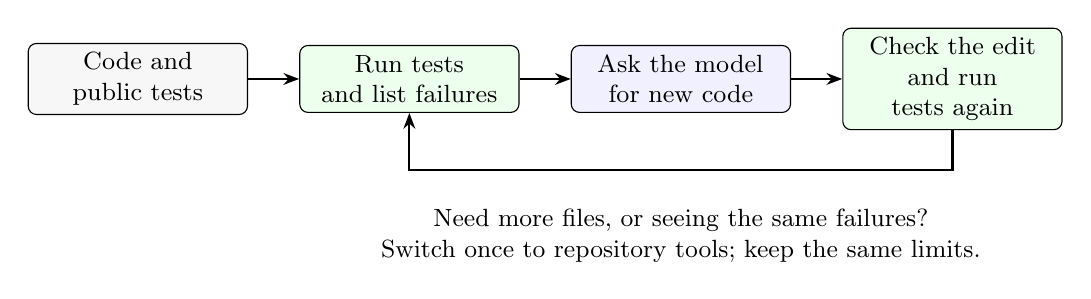
\begin{tikzpicture}[node distance=0.65cm]
\node[box] (a) {Code and\\public tests};
\node[box,right=of a,fill=green!7] (b) {Run tests\\and list failures};
\node[box,right=of b,fill=blue!6] (c) {Ask the model\\for new code};
\node[box,right=of c,fill=green!7] (d) {Check the edit\\and run tests again};
\draw[arr] (a)--(b);
\draw[arr] (b)--(c);
\draw[arr] (c)--(d);
\draw[arr] (d.south)--++(0,-0.5)-|(b.south);
\node[below=1.1cm of c,font=\small,align=center] (e)
{Need more files, or seeing the same failures?\\
Switch once to repository tools; keep the same limits.};
\end{tikzpicture}
\caption{The paid lean repair loop. Known verification steps are controlled by software,
not selected anew by the model. The model still performs code generation.
Private grading happens separately after the final candidate is frozen.}
\label{fig:overview}
\end{figure*}

\section{Method in Plain Terms}
\subsection{What the user provides}
For \texttt{solve}, the user supplies an existing Git repository, a task description, a list of
Python files that may change, and a public test command. Other files can be
included as read-only context, but they are not required for a minimal setup.
Time and request limits prevent the controller from retrying indefinitely.

The output is the edited code and a JSON run record. After a repair, a
\emph{verified} result means that the configured public checks passed.
It does \textbf{not} mean that all possible inputs, hidden tests or unstated
requirements are correct. Tests and other non-editable files are protected.

\subsection{A minimal repair setup: three steps}
\label{sec:setup}
The user does not need to configure a new agent, write a system prompt or
install a plugin. Install and sign in to Copilot CLI or Agency once, then
use the following steps from the cloned controller directory. The README
provides the CLI installation and sign-in commands.

\noindent\textbf{Step 1: install the controller.}\par
\begin{lstlisting}
.\setup.ps1
\end{lstlisting}
This installs the Python package and its checking tools. It does not install
or sign in to either coding CLI.

\noindent\textbf{Step 2: save a small task file.}\par
For an existing Git repository at \texttt{C:\textbackslash work\textbackslash project},
save the following as \texttt{task.json} in the controller directory:
\begin{lstlisting}
{
  "repo": "C:\\work\\project",
  "implementation_files": ["src/logic.py"],
  "working_tests": "python -m pytest -q tests",
  "backend": "copilot"
}
\end{lstlisting}
There are only four choices here: where the task repository is, which code
may change, how to run its public tests, and which CLI to call. Replace the
example paths and test command with those of the actual task. The task's
Python dependencies must be available to that test command.
For a separate project environment, use its absolute interpreter path:
\texttt{solve} resolves bare \texttt{python} to the controller's environment.

Use \texttt{"backend": "agency"} to choose Agency instead. The controller
looks for the CLI automatically; if it cannot find it, provide
\texttt{copilot\_exe} or \texttt{agency\_exe} with its full installed path.
No other configuration is required for this example.

\noindent\textbf{Step 3: ask for the repair.}\par
\begin{lstlisting}
.\verify-and-repair.ps1 solve --config task.json `
  --task "Fix the failing boundary case"
\end{lstlisting}
The controller runs the checks, requests a repair, and checks the result.
It prints the outcome and the path to the JSON record. By default, records
are saved beside the task repository, not inside it.
\textbf{This step uses paid model quota and may edit the allowed code.}

\paragraph{Defaults and optional settings.}
The default model is \texttt{gpt-6.1-sol} with medium reasoning. Limits are
600 seconds, three CLI sessions, 30 requests checked between sessions, and
180 seconds of checking time. These defaults need not be copied into the
task file. To use the model measured in our evaluation, add
\texttt{"model": "mai-code-2"}, provided the account has access.
Extra context files, linting, type checking and contracts are optional;
they are not prerequisites for using the basic loop.
Checks-only use needs the controller installation but neither a repair task
file nor a signed-in coding CLI; see Section~\ref{sec:normal-agent}.

\subsection{Only two pieces of notation}
Let $P$ mean the current code, and let $F$ mean its normalized public
failures. A failure records the check name, outcome and diagnostic.
For example:
\[
F=\{\texttt{test\_inc},\texttt{test\_double}\}.
\]
Before comparing failures, the controller removes changing details such as
local paths, timings and line numbers. It keeps useful details such as
assertion values. A timing change alone should not trigger another repair.
This comparison is a practical rule, not a proof that two failures have
the same cause.

\subsection{What changes after a repair?}
After each edit, the controller compares failures before and after the edit:
\begin{description}
\item[Resolved:] failed before, but no longer fails.
\item[Remaining:] failed before and still fails.
\item[New:] did not fail before, but fails now.
\end{description}
This short summary is the \emph{evidence delta}. The next model request gets
this summary instead of another full log. On the first request, all observed
failures are listed as new because there is no previous attempt to compare.

\begin{algorithm}[t]
\small
\caption{Lean repair with automatic tools fallback}
\label{alg:lean}
\KwIn{Code, task, allowed files, public checks, budgets}
\KwOut{Final code and an execution record}
Check setup before starting the measured clock\;
Start in \textnormal{source} mode; the sent-failures lists are empty\;
\While{time and action limits allow another step}{
  Run public checks on the actual code\;
  Record resolved, remaining and new failures for the last repair\;
  \If{a check cannot run reliably or protected files changed}{
    \Stop with an explicit error\;
  }
  \If{a repair was applied and the public success rule is met}{
    \Return code marked \textnormal{publicly verified}\;
  }
  Summarize the current failures as $F$\;
  \If{in source mode and tools are needed}{
    Switch permanently to tools mode\;
  }
  \If{$F$ was already sent in the current mode}{
    \Stop: the same failures were already tried in this mode\;
  }
  \If{no model session or request allowance remains}{
    \Stop: budget exhausted\;
  }
  Remember $F$ for the current mode\;
  Ask the selected CLI for one repair using public context\;
  Read the CLI's actual usage and update the limits\;
  \eIf{in source mode}{
    Validate and apply the source response
      (Algorithm~\ref{alg:apply})\;
  }{
    Inspect the resulting workspace for protected changes\;
  }
}
\Stop with the recorded termination reason\;
\end{algorithm}

\subsection{When the model gets another source attempt}
Source mode exposes no tools to the model. The prompt contains the allowed
implementation, read-only context and evidence delta. The model returns
complete replacement files in a fixed JSON format.

If a repair removes one failure but another remains, the evidence changed.
Another source request may therefore be useful, provided budgets remain.
Changing code without changing the failures is not enough to justify
another attempt in the same mode.

\subsection{When tools become necessary}
The controller switches to repository tools when context exceeds its size
limit, the source response is rejected, the model requests exploration,
or the same failures have already been tried in source mode. For example,
the model can return \texttt{\{"needs\_exploration":true\}} instead of guessing.
That object is not applied as source code; it triggers escalation through
the rejected-source path.

There is no switch back to source mode. The controller remembers failures
separately for source and tools. Consequently, unchanged evidence can justify
one stronger tools attempt, but cannot justify repeatedly running that mode.
Every attempt shares the same budgets.

\section{Worked Examples}
\subsection{Example 1: a small arithmetic defect}
Suppose the task is ``return the input plus one.'' The existing function is:
\begin{lstlisting}[language=Python]
def inc(x: int) -> int:
    return x - 1
\end{lstlisting}
The protected public examples are:
\begin{lstlisting}[language=Python]
assert inc(0) == 1
assert inc(-2) == -1
assert inc(9) == 10
\end{lstlisting}
The first check fails. Lean supplies this code and the failure to the model
without giving it tools. The requested response is data:
\begin{lstlisting}
{"files": [{
  "path": "src/logic.py",
  "content": "def inc(x: int) -> int:\n    return x + 1\n"
}]}
\end{lstlisting}
The controller validates the response, applies it, then reruns the public
examples. If the completion gate passes, it stops. There was no need for the
model to choose a file-reading tool, construct a Git patch or run the tests.
Section~\ref{sec:running} reports a genuine execution of this example.

\subsection{Example 2: one fix is not the whole fix}
Suppose increment and doubling both fail:
\[
F_{\text{old}}=\{\texttt{test\_inc},\texttt{test\_double}\}.
\]
The first edit fixes increment but not doubling:
\[
F_{\text{new}}=\{\texttt{test\_double}\}.
\]
The next request is told:
\begin{lstlisting}
resolved:  ["test_inc"]
remaining: ["test_double"]
new:       []
\end{lstlisting}
The controller does not stop merely because some tests passed.
If the edit also introduces a type error, that error is included in
\emph{new}. This distinction avoids losing regressions inside a general
``repair failed'' message.

\subsection{Example 3: a missing helper needs exploration}
Assume the supplied function calls a helper that is not explained by the
available context. A source-only proposal may be unreliable. The model can
request exploration, or the controller can observe repeated source failures.
It then switches once to tools, which can inspect repository context and
repair allowlisted files.

Table~\ref{tab:fallback} shows an illustrative no-progress case. These steps
describe implemented behavior covered by tests, not three additional paid
experiments. If failures change during tool repair, a further tool session
may be eligible within budget.

\begin{table}[t]
\centering\small
\begin{tabular}{lll}
\toprule
Current route & Evidence & Controller decision\\
\midrule
Source, not tried & $\{a,b\}$ & Ask for source\\
Source, already tried & $\{a,b\}$ & Switch to tools\\
Tools, already tried & $\{a,b\}$ & Stop as stalled\\
\bottomrule
\end{tabular}
\caption{Do not resend the same failures in the same mode.
Switching to tools does not reset time or request limits.}
\label{tab:fallback}
\end{table}

\section{How the Implementation Works}
\subsection{Applying an edit safely}
The model returns whole files rather than a patch with line numbers.
The controller checks that every path is allowed and appears only once.
It also rejects malformed JSON, checks Python syntax, and makes sure that
the workspace has not changed since the request began. Only then does it
write the replacements and record a diff. These checks make edit application
more reliable; they do not prove that the repaired code is correct.

\begin{algorithm}[t]
\small
\caption{Validate a source proposal}
\label{alg:apply}
\KwIn{Model response, allowed paths, saved workspace state}
Reject a failed request or missing usage record\;
Check the CLI record: the source request must expose no tools\;
Parse the size-limited JSON response; reject duplicate keys\;
Require at least one file, with unique allowed paths\;
Prepare the replacements and check their Python syntax\;
\If{the workspace has changed since the request began}{
  Reject the response rather than overwrite newer work\;
}
Apply the validated replacements and record a local diff\;
Let public rechecking decide whether the repair worked\;
\end{algorithm}

\subsection{Important safety limits}
\paragraph{No identical request in the same mode.}
Before dispatching a repair, the controller remembers its normalized
failures in that mode's set. Later dispatches check that set. Therefore,
one normalized failure set is sent at most once in source mode and once in
tools mode during a run. The comparison can still mistake different failures
for the same one, or the same failure for a new one.

\paragraph{Only listed files may change during lean repair.}
The source writer changes only checked, allowed paths. This assumes a trusted
controller and filesystem; it does not defend against an attacker changing
files during a write. In tools mode, changes to protected eligible files are
detected after the tool runs. They are reported, not silently undone.

\paragraph{Private tests are not part of repair.}
The \texttt{solve} command runs no private evaluator. It sends only the public
context and results supplied by the user. The user must not put private test
data in those files or commands. The controller is not an operating-system
sandbox.

\paragraph{Time limits are practical, not exact deadlines.}
Action and session limits prevent unlimited retries. Commands have timeouts,
but stopping processes and saving records can take extra time.

\subsection{Agency and Copilot CLI}
The backend integrations share the same controller, public checks and response
validation. Agency is called through its \texttt{copilot} subcommand;
Copilot CLI is called directly. Each backend requires its own installation,
authentication and access to the requested model.

For source responses, native per-request evidence must confirm zero exposed
tools. Missing streamed evidence may be read from the durable session log.
Tool-execution or subagent-start events reject source-only generation.
For the Copilot fallback, exposed tools are restricted to built-in
read/search, editing and shell lifecycle tools, not web/MCP or delegation.
Automatic plugin discovery and inherited environment-wide blanket approval
are disabled in the child process. Managed policy and hooks still apply.

\subsection{A session is not a model request}
One CLI session can issue several model requests. The controller reads the
native top-level \texttt{modelMetrics[*].requests.count}; it does not count
launches as requests or double-count agent/provider breakdowns.
Missing or malformed request usage blocks further inference.

Session limits are checked before a new invocation. Request limits are
checked \emph{between sessions}; one session can overshoot and the record
reports the overrun. Native AIU is a usage measure, not a currency amount.
Preflight runs outside experimental timing. Optional public contracts can
strengthen a scoped claim, but unknown or timeout is not a proof.

\section{Normal Agent Work and Verification Checkpoints}
\label{sec:normal-agent}
\subsection{Broader work without widening the repair allowlist}
The optional custom agent retains ordinary capabilities: reading and
explaining code, creating implementation files and tests, scaffolding projects,
working in other languages, editing documentation and performing authorized
repository operations. These actions use the outer agent's normal tools and
permissions. They do not require a repair task file or an editable-file
allowlist. The target is the current session's workspace or worktree, not a
different checkout remembered from an earlier task.

In VS Code, the user selects the custom agent explicitly~\cite{vscode-agents}.
It can be installed at workspace or user scope; the setup skill can defer
repair configuration until needed. Other agents are unaffected.
Ordinary work and checking code remain distinct. Before testing an implementation
task, the user authorizes its repair scope and bounded child-model budget once.
Failed checks then trigger counterexample-driven repair without another prompt
for each attempt inside that budget. A code-related question or tests-only
request does not authorize paid repair. Table~\ref{tab:normal-routing}
summarizes the testing-stage policy.

\begin{table}[t]
\centering\small
\begin{tabular}{@{}p{0.36\columnwidth}p{0.59\columnwidth}@{}}
\toprule
User task or outcome & Integration behavior\\
\midrule
Explain, review or plan & Answer normally; do not run checks merely because code is mentioned.\\
Create or edit files & Use normal tools; verify when reaching the code-testing stage.\\
Run code checks & Invoke checks-only \texttt{verify}, even without a preceding edit.\\
Non-coding work & Use normal tools; no automatic verification.\\
Code-check failure & Automatically enter counterexample-driven \texttt{solve} within the task's approved budget.\\
Timeout or setup error & Diagnose the check setup, not a speculative code repair.\\
\bottomrule
\end{tabular}
\caption{Testing-stage routing for the selected normal-agent integration.
This is an instruction policy, not a file-save hook or a measured benchmark arm.}
\label{tab:normal-routing}
\end{table}

\subsection{Checks-only verification}
The new \texttt{verify} command executes selected project checks without
constructing a repair controller or calling a coding model. It requires an
existing project directory and an explicit check command, but no Git
repository, task JSON or implementation allowlist. Newly created files and
non-Python projects are checked by their own tools.

With the task environment active, run from the controller directory:
\begin{lstlisting}
.\verify-and-repair.ps1 verify `
  --repo C:\work\project `
  --working-tests "python -m pytest -q tests"
\end{lstlisting}
Use the actual project command, not this example blindly. Optional
\texttt{--lint-command} and \texttt{--typecheck-command} add checks; a build
can also be the primary command. All selected commands run, including after
a failure. The default timeout is 180 seconds \emph{per command}, unlike
\texttt{solve}'s aggregate verifier-time budget.

Verification preserves the caller's \texttt{PATH} and environment rather
than substituting the controller's Python. Activate the project environment
or provide its absolute interpreter path. Commands run without an implicit
shell; shell operators require an explicit, reviewed shell invocation.

The result records each command, exit code, outcome, duration and output.
Exit status is 0 when all checks pass, 1 when a command reports failure, and
2 for invalid verifier input, command startup errors or timeouts. A fresh JSON
artifact is saved outside the project; an explicitly supplied output path
must not already exist. No private evaluator is run, and success means only
that the selected checks passed.

\subsection{Testing-stage routing and budgeted counterexample repair}
The agent invokes \texttt{verify} only when actually running code checks
during implementation or in response to an explicit testing request.
A question about tests does not execute them. There is no verification on
every message, file creation, edit or save, and an explicit request not to
run checks is respected.

\begin{algorithm}[t]
\small
\caption{Normal-agent testing-stage policy}
\label{alg:normal-agent}
\KwIn{User task, current workspace and project instructions}
\KwOut{Normal work, check results and any approved repair result}
Agree once on the implementation task's repair scope and bounded budget\;
Perform the requested ordinary work with normal tools\;
\If{the task is not at a requested code-checking step}{
  \Return without invoking verification or repair\;
}
Select relevant checks and their working directory and environment\;
Run \texttt{verify}; record the actual check outcomes\;
\If{a timeout or check-setup error is observed}{
  \Return diagnostics without starting code repair\;
}
\If{all selected checks pass}{
  \Return the limited public-check success result\;
}
Record the public counterexamples from failed code checks\;
\If{task approval is absent or the task is unsupported by \texttt{solve}}{
  \Return without a paid repair; agree on any further normal work\;
}
Automatically run bounded lean repair on the generated code (Algorithm~\ref{alg:lean})\;
Recheck each repair and supply resolved, remaining and new counterexample evidence\;
Report its result; do not reset a stalled or exhausted budget without renewed approval\;
\end{algorithm}

The standalone checks-only command never itself escalates into \texttt{solve}.
The selected agent automatically invokes \texttt{solve} after failed
implementation checks under the task's existing approval. The controller reruns
public checks and supplies actual failing assertions and diagnostics, rather
than a generic request to try again. It sends compact evidence deltas after
each repair and suppresses repeated evidence per capability. No private
evaluator evidence is supplied to repair.
A paid repair still requires an existing Git repository and an exact allowlist
of eligible existing Python implementation files.
Files created during ordinary coding can be included once they exist.
Tests, configuration and other non-allowlisted files remain protected during
the repair. Unsupported repair tasks can instead use normal agent work with
the user's agreement; they are not a reason to forbid ordinary file creation.

\paragraph{Scope of the guarantee.}
The same-agent MCP interface exposes \texttt{begin\_repair\_task} and
\texttt{verify\_code}. A Codex, Claude Code, Cursor or other local tool-aware
harness generates code normally, receives public counterexamples and repairs
with its own model. The feedback server preserves evidence deltas, repeated
evidence suppression, declared public-file protection and per-session
wall/verifier-time and repair-round budgets across restarts. It never launches
a child coding model. Repair-round counts are not native model request counts;
the host owns its model accounting and permissions. This integration was not
evaluated in the historical benchmark.

The separation inside \texttt{verify} is implemented in code.
Algorithm~\ref{alg:normal-agent}, by contrast, describes the custom agent's
instructions: it is not an enforced router or permission boundary. Direct
CLI users can still explicitly invoke \texttt{solve}. Normal folder trust,
tool approvals and managed policies continue to apply.

\paragraph{Side effects and accounting.}
The verifier does not itself edit source or launch a coding model, but a
supplied command can modify files, contact a service or consume quota.
Commands must therefore be reviewed and authorized; their outputs and JSON
artifacts may contain private project data. Zero controller-started model
requests does not mean zero outer-chat usage or zero cost in arbitrary tests.
The extension does not make a new latency or AIU claim.

\section{Evaluation}
\subsection{Questions and protocol}
We ask whether lean reduces usage and coding time, what correctness tradeoff
accompanies it, and whether a localized/synthesis arm adds benefit.
The historical campaign used Agency with MAI Code 2, medium reasoning,
on all 164 HumanEval tasks in each of three arms: tools-first, lean, and
localized/synthesis. There were 492 final budgeted candidates, with rotated
arm ordering.

Each trial allowed 600 seconds wall time, three sessions, 30 requests checked
at session boundaries, 180 seconds aggregate verifier time and 24 actions.
These are final candidates after a bounded process, not necessarily
single-request generations.

\subsection{Public obligations and independent grading}
Public checks came from original docstrings and were frozen before inference.
Unusable or reference-disagreeing examples were labeled, not rewritten using
private expected values. There were usable examples for 66 tasks; the other
98 had import-only public checks.

Preflight confirmed that all 164 references passed and all 164 negative
controls failed. Final candidates were graded using pinned EvalPlus code in
a separate network-disabled Docker container with private data read-only.
HumanEval+ success requires both the original and expanded tests to pass.
The official untrusted-check function was not modified.

\paragraph{Staged grading disclosure.}
At the user's request, 331 completed candidates were graded before the
remaining 161 were coded. Previously graded candidates were not repaired
or rerun; their hashes were confirmed unchanged. The amendment is preserved.
This is full task coverage, not one uninterrupted blinded run.

\subsection{Results}
Table~\ref{tab:results} gives the complete results. Lean had the lowest AIU
and coding time, but tools-first passed one more HumanEval+ task.
The base HumanEval score alone would hide this distinction.

\begin{table*}[t]
\centering\small
\begin{tabular}{lrrrrrr}
\toprule
Historical arm & HumanEval & HumanEval+ & Sessions & Requests & Native AIU & Coding seconds\\
\midrule
Tools-first & 163/164 & 156/164 & 165 & 641 & 182.67248 & 5456.04 \\
Lean & 164/164 & 155/164 & 164 & 164 & 54.74155 & 3128.27 \\
Localized/synthesis & 163/164 & 154/164 & 180 & 230 & 69.09720 & 3696.90 \\
\bottomrule
\end{tabular}
\caption{All 164 tasks in each arm, Agency / MAI Code 2 / medium.
HumanEval+ means base and expanded tests both pass.
Coding time sums controller durations; it excludes preflight and private
grading, and is not end-to-end campaign elapsed time.}
\label{tab:results}
\end{table*}

Relative to tools-first, lean reduced requests by 74.4\%,
model input tokens by 91.1\%, native AIU by 70.0\%,
and summed coding time by 42.7\%. Combined accuracy decreased
by 0.61 percentage points, or one task.
AIU per combined-correct task was 1.171 for tools-first
and 0.353 for lean. These are aggregate descriptive ratios,
not prices or guarantees for a new task.

The task-level pairing is informative: both arms passed 154 tasks,
tools alone passed 2, lean alone passed 1, and both
failed 7. These observations do not establish equivalence or
non-inferiority: no repeated-seed analysis or prespecified accuracy margin
was collected.

\subsection{What the results do not show}
The normal-agent workflow, file creation and standalone \texttt{verify}
command were not exercised in the historical campaign. Its results concern
the frozen source-first repair protocol, not this later integration.
Ordinary agent-authored tests are also distinct from the campaign's frozen
public obligations and independent private grading.

Lean used 164 source sessions and zero tool sessions in the full campaign.
The measured savings therefore do not demonstrate the value of its fallback.
The localized arm used 16 tool sessions and applied zero local solver repairs.
Its context slicing, response format and synthesis differ together, so it is
not an isolated symbolic ablation. The production implementation does not
expose localized synthesis as a profile.

A separate earlier three-task Requests comparison solved 2/3 tasks in both
localized and tools-first arms. Localized reduced input tokens by 12.0\%
but used 5.25\% more AIU and 67.8\% more coding time; all localized trials
escalated. Those public-spec-augmented tasks used a controlled local HTTP/TLS
environment, not an untouched leaderboard setup. This negative evidence
cautions against generalizing the function-level efficiency result.

\section{A Concrete Running Example}
\label{sec:running}
We ran Example 1 through the current lean-only API using Copilot CLI,
MAI Code 2 and medium reasoning. This was a real model request, not a
mock backend or a manually applied solution.

From the implementation directory, with Copilot authenticated:
\begin{lstlisting}
.\examples\verify-and-repair-demo\run.ps1 `
  -Backend copilot
\end{lstlisting}
Alternatively, choose \texttt{-Backend agency}. The script creates a fresh
temporary repository, prints the original code, invokes lean, prints the
repaired code, and independently reruns the three public assertions.
It refuses an existing workspace. Running it incurs paid usage.

The actual edit changed \texttt{return x - 1} to \texttt{return x + 1}.
All three public examples passed. The measured trace was:
\begin{center}\small
\begin{tabular}{lr}
\toprule
Step & Duration\\
\midrule
Initial public check: fail & 206 ms\\
Copilot source repair: pass & 33050 ms\\
Public re-check: pass & 166 ms\\
Controller wall total & 36.61 s\\
\bottomrule
\end{tabular}
\end{center}
Native accounting reported 1 request in one session,
3,744 input tokens, 57 output tokens and
0.20145 AIU. Zero exposed tools was confirmed by native evidence;
it was not inferred from a missing tool-call count.

The JSON result recorded \texttt{visible\_checks\_only}, not hidden
correctness. No private evaluator ran. The example allows one session,
so it cannot demonstrate a second-session fallback. Normal product defaults
allow three sessions. Separate earlier smoke checks exercised both CLIs'
source and tools routes; these are integration checks, not a full Copilot
benchmark. A rerun may have different latency, usage or output.

\section{Limitations and Discussion}
\paragraph{Weak public gates.}
Import-only checks do not verify task behavior. The HumanEval savings can
reflect successful initial generation under weak gates rather than
effective multi-repair verification. Public acceptance alone is insufficient.

\paragraph{Limited causal and statistical scope.}
The study has one model, one campaign, no repeated-seed variance estimate and
a staged-grading amendment. Twenty tasks were previously observed in this
project; 144 were new to it, not necessarily unseen in pretraining.
We report a descriptive accuracy--efficiency tradeoff, not universal
superiority, statistical non-inferiority or a vendor comparison.

\paragraph{Repository tasks can differ.}
Large contexts, multi-file dependencies and full-source output costs may
reverse the result. Setup and specification effort also matter.
The Copilot integration has genuine smoke-test evidence, not 492 repeated
benchmark trials.

\paragraph{Trust boundary.}
Protected-file checks are not a sandbox or rollback. The caller must provide
public commands and context, and must understand the host's tool permissions,
hooks and policies.
Normal-agent routing is instruction-based, while checks-only execution can
inherit side effects from the selected commands. Neither layer proves that
newly authored tests are adequate or independent of the implementation.

\paragraph{Relation to prior systems.}
Agent-loop descriptions~\cite{codex,claude} explain iterative inference
and tool feedback. Lean moves known checks and application into an explicit
controller; it does not assert that other agents lack deterministic tools.
HumanEval~\cite{humaneval} and expanded EvalPlus checks~\cite{evalplus}
motivate reporting original and stronger-test results separately.

\paragraph{Next experiments.}
Stronger frozen public tests, repeated seeds, prespecified accuracy margins
and larger repository tasks would test generalization. Evaluating the new
normal-agent workflow requires accounting for outer coding, test authoring,
check execution and any approved child repair together. Automatic public-test
generation inside lean repair and broader synthesis remain out of scope;
ordinary agent test authoring is a separate capability, not an evaluated gate.

\section{Conclusion}
Lean repair uses models for code proposals and software for the surrounding
verification loop. It retries only with changed evidence and preserves
bounded repository-tool escalation. In the complete function-level campaign,
it substantially reduced measured usage and time, while tools-first solved
one more expanded-test task. This motivates an efficiency-oriented product
choice with explicit limits, rather than a claim that lean is best at
everything.
The normal-agent integration adds flexible file creation and ordinary tools
without relaxing the paid repair's allowlist. Checks-only verification is
invoked at testing checkpoints; failed implementation checks automatically
enter counterexample-driven repair within a task's approved budget.
This is a usability extension, not additional evidence for the measured savings.

\section*{Artifacts and Reproduction}
The streamlined repository includes installation instructions, runtime source
code, tests, the runnable example, checks-only verification, the optional
normal-workflow custom agent, and this editable \LaTeX{} source.
Algorithms are typeset with \texttt{algorithm2e}. Historical benchmark runners,
measurement receipts and native logs are retained separately; the public
repository is not a complete reproduction bundle for the historical campaign.

The frozen campaign code and protocol are distinct from later product
changes. Current code must not resume a campaign frozen to older hashes.
Repository terms permit personal evaluation only; broader use requires
written permission. This technical report is not a peer-reviewed publication.

\begin{thebibliography}{9}
\small
\raggedright
\bibitem{codex}
Michael Bolin. \emph{Unrolling the Codex agent loop.}
OpenAI, January 23, 2026.
\url{https://openai.com/index/unrolling-the-codex-agent-loop/}
\bibitem{claude}
Anthropic. \emph{How Claude Code works.}
\url{https://code.claude.com/docs/en/how-claude-code-works}
\bibitem{humaneval}
OpenAI. \emph{HumanEval: Hand-Written Evaluation Set.}
\url{https://github.com/openai/human-eval}
\bibitem{evalplus}
EvalPlus. \emph{Rigorous evaluation of LLM-synthesized code.}
\url{https://github.com/evalplus/evalplus}
Pinned commit: \texttt{26d6d00bb1fd0fa37f39c99d5290da67891d1c5e}.
\bibitem{copilot}
GitHub. \emph{Copilot CLI documentation} and installed CLI help.
\url{https://docs.github.com/en/copilot/how-tos/copilot-cli}
\bibitem{vscode-agents}
Microsoft. \emph{Custom agents in VS Code.}
\url{https://code.visualstudio.com/docs/agent-customization/custom-agents}
\end{thebibliography}
\end{document}
